\documentclass[11pt]{article}

\usepackage[utf8]{inputenc}
\usepackage[T1]{fontenc}
\usepackage{lmodern}
\usepackage{amsmath, amssymb, mathtools}
\usepackage{bm}
\usepackage{graphicx}
\usepackage{xcolor}
\usepackage{hyperref}
\usepackage[capitalize,noabbrev]{cleveref}
\usepackage{geometry}
\usepackage{caption}
\usepackage[numbers]{natbib}
\geometry{a4paper, margin=2.4cm}

\newcommand{\bxi}{\boldsymbol{\xi}}
\newcommand{\bx}{\bm{x}}
\newcommand{\avg}[1]{\langle #1 \rangle}
\newcommand{\e}{{\mathrm{e}}}
\newcommand{\dd}{{\mathrm{d}}}
\newcommand{\Bnet}{\beta_{\mathrm{net}}}
\newcommand{\phieq}{\phi_{\mathrm{eq}}}
\newcommand{\fret}{f_{\mathrm{ret}}}
\newcommand{\gmax}{g_{\max}}
\newcommand{\acGauss}{\alpha_c^{\mathrm{G}}}
\newcommand{\acBd}{\alpha_c^{\mathrm{bd}}}
\newcommand{\acSd}{\alpha_c^{\mathrm{sd}}}
\newcommand{\acSp}{\alpha_c^{\mathrm{sp}}}

\title{\bfseries Saddle-Dominated Capacity of the\\
LSE Dense Associative Memory}
\author{}
\date{}

\begin{document}
\maketitle

% =========================================================================
\begin{abstract}
\noindent
The log-sum-exp (LSE) Dense Associative Memory stores an exponentially
large set of patterns on the $N$-sphere with a kernel sharpness
parameter we call $\Bnet$.  \citet{ramsauer2021hopfield} obtained a
limiting storage load $\alpha_c = 1/2$ at zero temperature by modelling
the inter-pattern overlaps as Gaussian; their bound is independent of
$\Bnet$.  We revisit the calculation under the exact spherical overlap
density.  The dominant contribution to the noise floor moves from the
upper edge of the overlap distribution to an interior saddle of the
partition-sum integrand, with saddle value $\gmax(\Bnet)$.  This single
quantity controls every corrected boundary in the $(\alpha, T)$ plane.
At $T = 0$ the corrected capacity is $\Bnet - \gmax(\Bnet)$, the load
at which the cusp of the leading-order free energy reaches the unit
sphere and the retrieval basin disappears.  It is finite, depends on
$\Bnet$, sits below Ramsauer's bound at moderate $\Bnet$, and exceeds
it at large $\Bnet$.  Hybrid Monte Carlo at $N = 100$ places the
empirical basin boundary on the corrected curve, consistent with the
analytical prediction.
\end{abstract}

% =========================================================================
\section{Introduction}
\label{sec:intro}

The Hopfield network~\citep{Hopfield1982} stores patterns as minima of a
pairwise energy and retrieves the closest stored pattern from a noisy
cue.  Classical pairwise storage saturates at a load of about $0.138$
patterns per neuron~\citep{amit1987statistical}.  Dense Associative
Memory replaces the pairwise interaction by a strongly nonlinear energy
and raises the capacity to an exponential
$M = \e^{\alpha N}$~\citep{krotov2016dense, krotov2021large,
demircigil2017model}.  In the continuous version of the model, both the
stored patterns $\bxi^\mu \in \mathbb{R}^N$ and the chain $\bx$ live on
the sphere $|\bx|^2 = N$.  The log-sum-exp (LSE) variant of
\citet{ramsauer2021hopfield} writes
\begin{equation}
H(\bx) = -\Bnet^{-1} \ln \sum_{\mu=1}^{M}
   \exp\!\bigl(\Bnet\,\bx \cdot \bxi^\mu\bigr),
\label{eq:lse}
\end{equation}
with $\Bnet$ a kernel sharpness parameter that scales the dot product
inside the log-sum-exp.  $\Bnet$ controls how strongly the energy
distinguishes patterns and is independent of the simulation temperature
$T$.

For continuous LSE, \citet{ramsauer2021hopfield} derived a limiting
load $\alpha_c = 1/2$ at $T = 0$.  The argument treats the inter-pattern
overlap $\varphi_{1\mu} = \bxi^1 \cdot \bxi^\mu / N$ as a Gaussian with
mean $0$ and variance $1/N$, and asks at what load the typical maximum
of $M$ such overlaps first reaches $1$.  The Gaussian extreme value
satisfies $\varphi_{\max}^{(G)} = \sqrt{2\alpha}$, so the condition
$\varphi_{\max}^{(G)} = 1$ gives $\alpha = 1/2$.  The bound does not
involve $\Bnet$.

The Gaussian is the leading term of the exact spherical overlap density
near $\varphi = 0$, but the two densities diverge near $\varphi = 1$.
Whether the corrected density alters the capacity was raised by
\citet{icml2026theory}, who derived the finite-temperature retrieval
boundary $T_c(\alpha)$ for LSE and LSR under the Gaussian approximation
and flagged its noise-floor derivation as the candidate failure point.
\citet{iclr2026mc} subsequently measured this boundary by direct Monte
Carlo at moderate $N$ for both kernels, without pursuing the low-$T$
limit near the limiting load.  The compactly supported LSR variant was
analysed by \citet{petrova2026metastable} from a different angle: by
direct Monte Carlo at $N \approx 40$--$50$ they showed that the apparent
retrieval boundary in the simulations is a kinetic crossover.  A
metastable strip sits below the thermodynamic boundary, separated from
the competing-pattern basins by an entropic barrier whose Kramers escape
time grows exponentially in $N$.  They note that resolving the strip at
larger $N$ would require a smarter Monte Carlo scheme than the direct
method they employed, and do not provide one.

This paper revisits Ramsauer's $\alpha_c = 1/2$ for LSE under the exact
spherical density, treating $\Bnet$ as a free parameter.  The corrected
capacity is finite and depends on $\Bnet$; it sits below Ramsauer's
bound at moderate $\Bnet$, crosses it at $\Bnet \approx 0.7$, and grows
logarithmically with $\Bnet$ beyond.  Two boundary curves arise in the
$(\alpha, T)$ plane: a single-pattern spinodal $\acSp(\Bnet, T)$ at
which the cusp of the leading-order free energy reaches the basin
minimum and the basin disappears, and a thermodynamic crossover
$\acSd(\Bnet, T)$ at which the noise floor and the basin minimum
exchange order in free energy.  Both curves are set by the integrand
saddle value $\gmax(\Bnet)$, and they coincide at $T = 0$ at the
endpoint $\Bnet - \gmax(\Bnet)$.  At $T > 0$ they separate; the
spinodal is the relevant boundary for cold-initialised Monte Carlo,
the saddle line is the thermodynamic crossover.

Two technical points motivate the rest of the paper.  First, the naive
correction — replacing the Gaussian by the exact density and applying
the same right-edge logic — gives the wrong capacity: the LSE partition
sum is governed by an interior saddle, not by the edge of the overlap
distribution.  Second, the local-refresh Monte Carlo schemes used to
accelerate large-$N$ studies fail near the capacity boundary by
introducing unquenched disorder; the simulations in this paper rely on a
hybrid scheme that keeps the cusp-tail patterns explicit while treating
the bulk analytically.

\Cref{sec:theory} develops the theory: the Gaussian baseline, the naive
exact-density variant, the interior saddle, the cusp picture, the
spinodal, and the two-protocol picture.  \Cref{sec:mc} describes the
three Monte Carlo schemes (direct, truncated, hybrid) used here, with a
paragraph on why local refresh fails.  \Cref{sec:results} shows the
empirical $N = 100$ heatmap together with the four boundary curves.
\Cref{sec:discussion} closes with the Ramsauer claim and the
saddle-vs-spinodal distinction.

% =========================================================================
\section{Theory}
\label{sec:theory}

\paragraph{Setup.}
Both the stored patterns $\bxi^\mu$ and the chain $\bx$ lie on the
sphere $S^{N-1}(\sqrt N)$.  The inter-pattern overlap
$\varphi_{1\mu} = \bxi^1 \cdot \bxi^\mu / N$ between a fixed retrieving
pattern and a random spurious one is the projection of one uniform
direction onto another; its density on $[-1, 1]$ is the spherical
density
\begin{equation}
f(\varphi) = C_N\,(1 - \varphi^2)^{(N-3)/2},
\qquad
C_N = \frac{\Gamma(N/2)}{\Gamma((N-1)/2)\sqrt\pi}\,.
\label{eq:fphi}
\end{equation}
At large $N$, $f$ concentrates near $\varphi = 0$ with variance $1/N$,
but its right tail near $\varphi = 1$ decays as $(1-\varphi^2)^{N/2}$,
lighter than any Gaussian of matched variance.  The chain-target overlap
$\varphi_1 = \bxi^1 \cdot \bx / N$ measures retrieval.

For a chain in the basin of $\bxi^1$ the LSE log-sum is dominated by the
$\mu = 1$ term, $H(\bx)/N \approx -\Bnet^{-1} \ln \e^{\Bnet N \varphi_1}
= -\varphi_1$ — the $\Bnet$ factor inside the exponential and the
$\Bnet^{-1}$ in front of the logarithm cancel for any single-term
dominant contribution.  Adding the perpendicular-subspace entropy
$s(\varphi_1) = \tfrac12 \ln(1 - \varphi_1^2)$ and minimising
$f = u - Ts$ with $u = 1 - \varphi_1$ gives the retrieval free energy
per spin
\begin{equation}
\fret(T) = (1 - \phieq) - \tfrac{T}{2} \ln(1 - \phieq^2),
\qquad
\phieq(T) = \tfrac12\bigl(-T + \sqrt{T^2 + 4}\bigr),
\label{eq:fret}
\end{equation}
$\Bnet$-independent by the same cancellation.

Away from the basin the noise floor comes from the $M-1$ spurious sum
\begin{equation}
S(\bx) \;=\; \sum_{\mu \neq 1} \e^{\Bnet N \varphi_\mu(\bx)},
\qquad
\frac{1}{N}\ln S
\;\approx\; \alpha + \frac{1}{N}\ln\!\int_{-1}^{1} f(\varphi)\,
            \e^{N \Bnet \varphi}\,\dd\varphi,
\label{eq:S}
\end{equation}
where we used $M = \e^{\alpha N}$ and replaced the sum over patterns by
an integral with density $f$ — valid in the bulk of $\bx$ because the
$\varphi_\mu$ are independent draws from $f$.  The integrand exponent is
$g(\varphi; \Bnet) = \tfrac12 \ln(1 - \varphi^2) + \Bnet\,\varphi$.

\paragraph{Gaussian baseline.}
Replacing $f$ by the moment-matched Gaussian
$\sqrt{N/2\pi}\,\e^{-N\varphi^2/2}$ makes the exponent
$-\tfrac12 \varphi^2 + \Bnet\varphi$ monotone in $\varphi$ on $[-1,1]$
for $\Bnet \le 1$, so the integral~\eqref{eq:S} is set by the typical
extreme of $M$ Gaussian samples, $\varphi_{\max}^{(G)} = \sqrt{2\alpha}$.
Substituting gives $N^{-1}\ln S \to \Bnet \sqrt{2\alpha}$ and a
noise-floor energy per spin
$u_{\mathrm{noise}}^{(G)} = 1 - \sqrt{2\alpha}$.  The boundary
$u_{\mathrm{noise}}^{(G)} = \fret(T)$ reads
\begin{equation}
\acGauss(T) = \tfrac12\bigl[1 - \fret(T)\bigr]^2,
\qquad \acGauss(0) = \tfrac12.
\label{eq:acgauss}
\end{equation}
The $\Bnet^{-1}$ prefactor of $H$ and the $\Bnet$ inside the exponent
cancel each other at the right edge, so~\eqref{eq:acgauss} is
$\Bnet$-independent.  This is Ramsauer's bound.

\paragraph{Naive correction: exact density at the edge.}
Keep the exact density $f$ but apply the same edge logic.  The typical
maximum of $M$ samples from $f$ satisfies
$M\Pr_f(\varphi > \varphi_{\max}) = 1$, which after computing the right
tail of~\eqref{eq:fphi} gives
$\varphi_{\max}(\alpha) = \sqrt{1 - \e^{-2\alpha}}$.  The exponent at
the edge is $g(\varphi_{\max}) = -\alpha + \Bnet\,\varphi_{\max}$, so
$N^{-1}\ln S \to \Bnet\,\varphi_{\max}(\alpha)$ and
$u_{\mathrm{noise}}^{(\mathrm{ex})} = 1 - \varphi_{\max}(\alpha)$.
Solving $u_{\mathrm{noise}}^{(\mathrm{ex})} = \fret(T)$ yields
\begin{equation}
\acBd(T) \;=\; -\tfrac12 \ln\!\bigl[1 - (1 - \fret(T))^2\bigr],
\qquad \acBd(0) = +\infty.
\label{eq:acbd}
\end{equation}
The boundary diverges at $T = 0$: the exact density has no finite right
edge, so the edge logic returns no bound.  This is the right answer for
the compactly supported LSR kernel — there the kernel cuts the integral
off at a finite $\varphi_c < 1$~\citep{petrova2026metastable}.  For LSE
the edge logic is wrong whenever the integrand has an interior maximum
inside $[0, 1)$.

\paragraph{Interior saddle: the correct boundary.}
The exponent $g(\varphi; \Bnet)$ has derivative
$g'(\varphi) = \Bnet - \varphi/(1 - \varphi^2)$, which vanishes at the
positive root
\begin{equation}
\varphi^{*}(\Bnet) = \frac{-1 + \sqrt{1 + 4\Bnet^2}}{2\Bnet}\,.
\label{eq:phistar}
\end{equation}
The saddle is inside $(0, 1)$ for every $\Bnet > 0$.  By Laplace's
method,
\begin{equation}
\int_{-1}^{1} f(\varphi)\,\e^{N\Bnet\varphi}\,\dd\varphi
\;\sim\; \sqrt{\frac{2\pi}{N\,|g''(\varphi^{*})|}}\,
        \e^{N\,\gmax(\Bnet)},
\qquad
\gmax(\Bnet) \;\equiv\; g(\varphi^{*}; \Bnet)
   \;=\; \tfrac12 \ln(1 - \varphi^{*\,2}) + \Bnet\,\varphi^{*},
\label{eq:gmax}
\end{equation}
so $N^{-1}\ln S \to \alpha + \gmax(\Bnet)$ and the noise-floor energy
per spin reads $u_{\mathrm{noise}}^{(\mathrm{sd})}
= 1 - [\alpha + \gmax(\Bnet)]/\Bnet$.  Equating this to $\fret(T)$ gives
the saddle-dominated boundary
\begin{equation}
\boxed{\;
\acSd(\Bnet, T) \;=\; \Bnet\,[1 - \fret(T)] - \gmax(\Bnet).
\;}
\label{eq:acsd}
\end{equation}
The dependence on $\Bnet$ is real.  At the right edge, the same $\Bnet$
factor appears in retrieval and noise floor and cancels — that is why
Ramsauer's bound is $\Bnet$-independent.  At the interior saddle the
location $\varphi^{*}(\Bnet)$ itself shifts with $\Bnet$, and the
cancellation breaks.  \Cref{fig:beta-curve} shows
$\acSd(\Bnet, 0) = \Bnet - \gmax(\Bnet)$ together with Ramsauer's
$\acGauss = 1/2$.  $\acSd(\Bnet, 0)$ crosses Ramsauer's flat line at
$\Bnet \approx 0.7$: below this value the corrected capacity is more
restrictive than Ramsauer's, above it more permissive.  The endpoints are explicit: as $\Bnet \to 0$,
$\varphi^{*} \to \Bnet$ and $\gmax \to \Bnet^2/2$, giving the linear
$\acSd(\Bnet, 0) \to \Bnet$; as $\Bnet \to \infty$, $\varphi^{*} \to
1 - 1/(2\Bnet)$ and $\gmax \to \Bnet - \tfrac12(\ln \Bnet + 1)$, giving
the logarithmic growth $\acSd(\Bnet, 0) \to \tfrac12(1 + \ln \Bnet)$.
The Monte Carlo simulations of \Cref{sec:mc,sec:results} fix $\Bnet = 1$
for the numerics, where $\acSd(1, 0) \approx 0.6226$.

\begin{figure}[t]
\centering
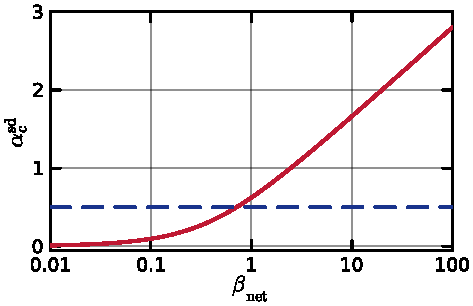
\includegraphics[width=90mm,height=60mm]{panels_paper/alpha_c_vs_beta.pdf}
\caption{Zero-temperature capacity $\acSd(\Bnet, 0)$~\eqref{eq:acsd}
of the LSE DAM as a function of the kernel sharpness $\Bnet$ (red),
together with Ramsauer's $\Bnet$-independent
bound $\acGauss = 1/2$~\eqref{eq:acgauss} (blue dashed).}
\label{fig:beta-curve}
\end{figure}

\paragraph{Cusp picture.}
The saddle integral~\eqref{eq:gmax} is independent of $\bx$: by isotropy
of the random patterns, after averaging over the directions orthogonal
to $\bxi^1$ only $\varphi_{1\mu}$ — not $\bx$ itself — enters the
spurious sum.  The chain therefore competes inside the LSE logarithm
between the retrieval term $\e^{\Bnet N \varphi_1}$ and an
$\bx$-independent bulk $S \sim \e^{N[\alpha + \gmax(\Bnet)]}$.  At large
$N$,
\begin{equation}
\Bnet^{-1} \ln\!\bigl[\e^{\Bnet N \varphi_1} + S\bigr]
\;\to\; \max\!\bigl(\varphi_1,\;\varphi_c(\alpha, \Bnet)\bigr),
\qquad
\varphi_c(\alpha, \Bnet) \;=\; \frac{\alpha + \gmax(\Bnet)}{\Bnet}\,,
\label{eq:cusp}
\end{equation}
and the leading-order free energy per spin is
\begin{equation}
\frac{F(\varphi_1; T, \alpha, \Bnet)}{N}
\;=\; -\max\!\bigl(\varphi_1, \varphi_c\bigr)
   \;-\; \tfrac{T}{2}\ln(1 - \varphi_1^2).
\label{eq:F-LO}
\end{equation}
The two branches meet in a cusp at $\varphi_1 = \varphi_c$.  We call the
right branch (slope $-1$) the \emph{retrieval basin}: for $\varphi_1 >
\varphi_c$ the retrieval term dominates the log-sum and the chain feels
the linear pull of $\bxi^1$.  We call the left branch (zero energy
slope) the \emph{saddle valley}: for $\varphi_1 < \varphi_c$ the bulk
saddle dominates the log-sum, the energy in $\varphi_1$ is flat, and the
sphere entropy $-(T/2)\ln(1-\varphi_1^2)$ alone pulls the chain toward
$\varphi_1 = 0$.  \Cref{fig:cusp} plots~\eqref{eq:F-LO} at $\alpha =
0.5$, $\Bnet = 1$, $\varphi_c \approx 0.877$.

\begin{figure}[t]
\centering
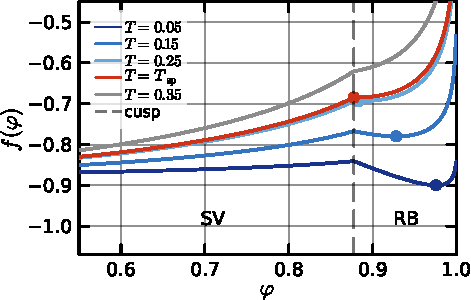
\includegraphics[width=90mm,height=60mm]{panels_paper/cusp_illustration.pdf}
\caption{Leading-order free energy per spin $F(\varphi_1)/N$
from~\eqref{eq:F-LO} at $\alpha = 0.5$, $\Bnet = 1$, for five
temperatures.  The dashed vertical line marks the cusp
$\varphi_c = \alpha + \gmax \approx 0.877$ separating the saddle valley
on the left from the retrieval basin on the right.  Dots: basin minima
$\phieq(T)$.  At $T = T_{\mathrm{sp}}(0.5, 1) \approx 0.262$ the basin
minimum reaches the cusp; for $T = 0.35 > T_{\mathrm{sp}}$ the basin no
longer exists (grey curve).}
\label{fig:cusp}
\end{figure}

\paragraph{Single-pattern spinodal.}
The retrieval branch has a local minimum at $\phieq(T)$ from
$\eqref{eq:fret}$, valid only while $\phieq(T) > \varphi_c$.  As $T$
rises, $\phieq(T)$ drops; when it reaches $\varphi_c$ the local minimum
disappears and the chain slides to $\varphi_1 = 0$.  The condition
$\phieq(T) = \varphi_c$ defines the single-pattern spinodal
\begin{equation}
\acSp(\Bnet, T) \;=\; \Bnet\,\phieq(T) - \gmax(\Bnet),
\qquad
T_{\mathrm{sp}}(\alpha, \Bnet)
   \;=\; \frac{\Bnet^2 - (\alpha + \gmax(\Bnet))^2}
              {\Bnet\,(\alpha + \gmax(\Bnet))}\,.
\label{eq:acsp}
\end{equation}
At $T = 0$, $\phieq(0) = 1$, and the two curves~\eqref{eq:acsd}
and~\eqref{eq:acsp} share the same endpoint
$(\Bnet - \gmax(\Bnet),\,0)$.

\paragraph{Two boundaries, two protocols.}
At $T > 0$ the spinodal $\acSp$ and the thermodynamic crossover
$\acSd$ separate, with $\acSd < \acSp$ (since
$\acSp - \acSd = -(T/2)\ln(1 - \phieq^2) > 0$).  In the strip
$\acSd(\Bnet, T) < \alpha < \acSp(\Bnet, T)$ the basin still exists and
lies above the cusp, but the bulk noise floor is lower in free energy.
The escape barrier the chain must cross to leave the basin,
$\Delta F_{\mathrm{esc}}/N
   = (\phieq - \varphi_c) + (T/2) \ln[(1 - \phieq^2)/(1 - \varphi_c^2)]$,
depends only on $\phieq - \varphi_c$ and vanishes at $\acSp$, not at
$\acSd$.  The Kramers escape time
$\tau \sim \exp(N\,\Delta F_{\mathrm{esc}}/T)$ therefore grows
exponentially with $N$ throughout $\alpha < \acSp$, regardless of which
side of $\acSd$ we are on.  Consequently:

\begin{itemize}
\item In the equilibrium (infinite-time) protocol, the chain
Boltzmann-distributes between the basin and the noise floor; the
empirical boundary is $\acSd$, the free-energy crossover.
\item In the cold-initialised, finite-budget protocol — the practical
retrieval scheme — the chain stays in the basin until its first Kramers
escape.  The asymptotic boundary at $N \to \infty$ is the spinodal
$\acSp$, since $\tau \to \infty$ throughout $\alpha < \acSp$.  At
finite $N$ the empirical boundary is the Kramers contour
$\tau(\alpha, T, N) = T_{\mathrm{MC}}$, which lies inside the strip
$\acSd < \alpha < \acSp$ and drifts toward $\acSp$ as $N$ grows.
\end{itemize}

At $T = 0$ both curves coincide at $\Bnet - \gmax(\Bnet)$ and the
distinction disappears.  \Cref{fig:tau} confirms the picture at
$N = 100$: $\log_{10} \avg\tau$ at five $\alpha$ approaching the
$T = 0$ endpoint $0.6226$ shows the basin surviving the full budget
$10^6$ MC steps at low $T$ and dropping by several orders of magnitude
over a $T$ window of width $\sim 0.01$ that slides toward $T = 0$ as
$\alpha$ rises.  A Kramers fit
$\avg\tau \sim \tau_0\,\e^{c\Delta F/T}$ predicts that the product
$T \log\avg\tau$ reads off the effective barrier $c\Delta F$; in our
data this product traces a shallow $U$ in $T$ at each $\alpha$ — a
finite high-$T$ prefactor on one side and a $T$-dependent barrier on
the other ($\phieq(T) - \varphi_c$ shrinks as $T$ rises).  The minimum
value of $T \log_{10}\avg\tau$ drops monotonically from
$\approx 0.56$ at $\alpha = 0.50$ to $\approx 0.16$ at $\alpha = 0.58$
and below the measurement floor at $\alpha = 0.60$, consistent with the
effective barrier vanishing as the spinodal is approached.

\begin{figure}[t]
\centering
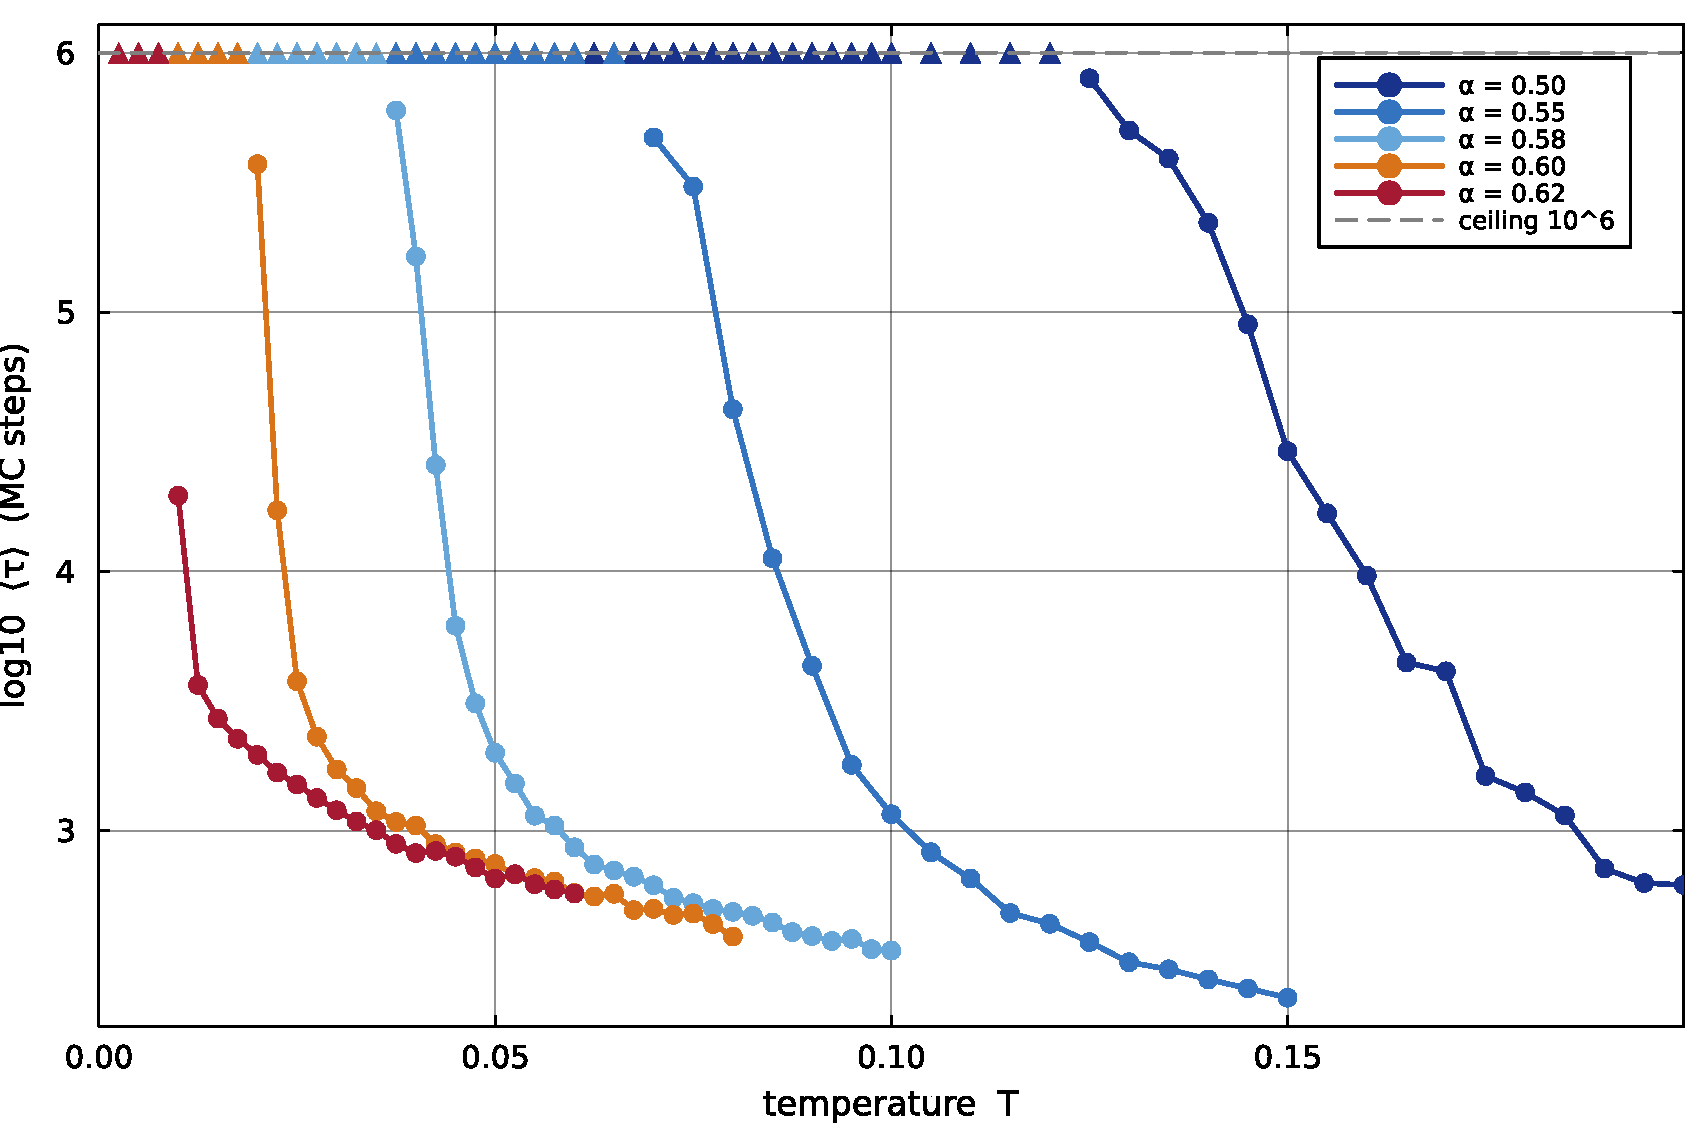
\includegraphics[width=0.82\linewidth]{panels_paper/log_tau_vs_T_N100_Ndim.pdf}
\caption{Mean basin escape time $\avg\tau$ versus $T$ at $N = 100$ from
N-dim hybrid MC, $32$ disorder samples per cell, $\Bnet = 1$.  Five
values of $\alpha$ approaching $\acSd(1, 0) \approx 0.6226$.  Cells in
which no disorder escaped within $10^6$ MC steps are not shown; the grey
dashed line marks that budget ceiling.  The escape window narrows and
slides toward $T = 0$ as $\alpha$ rises.}
\label{fig:tau}
\end{figure}

% =========================================================================
\section{Monte Carlo schemes}
\label{sec:mc}

We use three Metropolis variants on $\bx \in \sqrt N \cdot S^{N-1}$,
all at $\Bnet = 1$.  They differ in how they treat the $M = \e^{\alpha
N}$ patterns inside the LSE log-sum.

\paragraph{Direct.}
All $M$ patterns are stored explicitly and the log-sum is evaluated over
all of them at every step.  Cost per step $\sim M N$.  Direct MC is
feasible up to $N \approx 25$ at $\alpha = 0.7$
($M \approx 4 \times 10^7$); it is impossible at $N = 100$, $\alpha =
0.6$, where $M \approx 10^{26}$ exceeds available memory by twenty
orders of magnitude.

\paragraph{Truncated.}
For each disorder draw we sample the $K \sim 10^4$ patterns whose
overlap with $\bxi^1$ exceeds a cutoff $\varphi_{\mathrm{keep}}$.  The
cutoff is chosen so that the expected count above it equals the budget
$K$.  The remaining $M - K$ patterns below the cutoff enter the LSE
log-sum through an analytic constant
$\ln C_{\mathrm{bulk}} = \alpha N + \ln \int_{-1}^{\varphi_{\mathrm{keep}}}
f(\varphi)\,\e^{N\varphi}\,\dd\varphi$.  The retained set is fixed once
per disorder.  At $N = 25$ truncated and direct produce the same basin
boundary across the full $\alpha$ range we measure, so the discarded
patterns are genuinely outside the basin physics rather than silently
dropped.  Truncated is the workhorse for the wide heatmap in
\Cref{sec:results}.

\paragraph{Hybrid.}
Same decomposition as truncated, with two changes: the cutoff is set at
the cusp position $\varphi_c(\alpha, \Bnet)$ from~\eqref{eq:cusp} rather
than chosen by budget, and the bulk integral is replaced by its
saddle-point value $M\,\e^{N\gmax(\Bnet)}$ — an $\bx$-independent
constant inside the log-sum.  Patterns above $\varphi_c$ are drawn from
the spherical density~\eqref{eq:fphi} restricted to $\varphi > \varphi_c$.
In the rescaled variable $y = (1 + \varphi)/2 \in [0, 1]$, the spherical
density becomes a symmetric Beta:
\begin{equation}
y \sim \mathrm{Beta}\!\Bigl(\tfrac{N-1}{2}, \tfrac{N-1}{2}\Bigr)
   \;\;\text{truncated to}\;\; y \in \bigl[(1 + \varphi_c)/2,\,1\bigr],
\qquad \varphi_{1\mu} = 2y - 1.
\label{eq:beta-tail}
\end{equation}
Each retained pattern is then assembled from its $\varphi_{1\mu}$ and a
uniform direction $u_\mu$ on the $(N-2)$-sphere perpendicular to
$\bxi^1$.  At the loads and dimension studied here ($N = 100$,
$\alpha \in [0.5, 0.62]$), the expected count of overlaps above
$\varphi_c$ is below unity for every $\alpha$, so the algorithm
typically retains only $\bxi^1$ explicitly and treats every other
pattern through the bulk constant.  This is a faithful sampler of the
leading-order free energy~\eqref{eq:F-LO}: below the cusp the bulk
constant inside the log-sum collapses $\Bnet^{-1}\ln[\cdot]$ to the
constant $\varphi_c$ — the noise-floor branch — but the chain still
feels the sphere geometry through the entropy term $-(T/2)\ln(1 -
\varphi_1^2)$, which is what drives the slide to $\varphi_1 = 0$.

\paragraph{Why local refresh fails.}
A faster scheme — sometimes called ``smart'' — refreshes the retained
set every $N_{\mathrm{refresh}}$ steps from a cone around the current
chain position, keeping only the patterns whose overlap with $\bx$ is
currently large.  The refresh breaks the quenched-disorder assumption
that underlies~\eqref{eq:fret}--\eqref{eq:acsd}.  As $\bx$ wanders, new
patterns are minted at every refresh, so the cumulative set of patterns
seen along a single trajectory exceeds $M$, and the chain effectively
faces a denser pattern set than the model defines.  In the retrieval
basin the spurious-recruitment rate alone destroys retrieval — for
reasons unrelated to~\eqref{eq:acsd}.  Truncated and hybrid both fix the
retained set once per disorder and avoid the issue.

% =========================================================================
\section{Results}
\label{sec:results}

\Cref{fig:heatmap} shows $\avg{\varphi_1} - \phieq(T)$ over the
$(\alpha, T)$ plane at $\Bnet = 1$.  The bulk of the plane,
$\alpha \in [0.20, 0.70]$, uses truncated MC at varying $N$ (the load
$M = \e^{\alpha N}$ is held fixed at $M \approx 4.4 \times 10^6$ by
ramping $N$ with $\alpha$).  A fine $T$-grid hybrid MC at $N = 100$
fills in the rectangle $\alpha \in [0.5, 0.62]$, $T \in [0, 0.10]$.

The basin region (white) is bounded by a sharp dark-red transition that
pinches at $\alpha \approx 0.6226$ at $T = 0$.  Ramsauer's
$\acGauss = 1/2$ from~\eqref{eq:acgauss} and the exact-edge curve
$\acBd$ from~\eqref{eq:acbd} both sit visibly off the empirical
boundary at low $T$.  The thermodynamic crossover $\acSd$
from~\eqref{eq:acsd} (red) and the spinodal $\acSp$
from~\eqref{eq:acsp} (purple) bound a strip
$\acSd < \alpha < \acSp$ at $T > 0$, sharing the single endpoint at
$T = 0$.  The empirical line at $N = 100$ sits inside this strip, on
the Kramers contour $\tau(\alpha, T, N) = T_{\mathrm{MC}}$ where the
chain escapes within the simulation budget.  As $N$ grows the contour
drifts toward $\acSp$ — the cold-initialised asymptotic boundary
discussed in \S\ref{sec:theory}.

\begin{figure}[t]
\centering
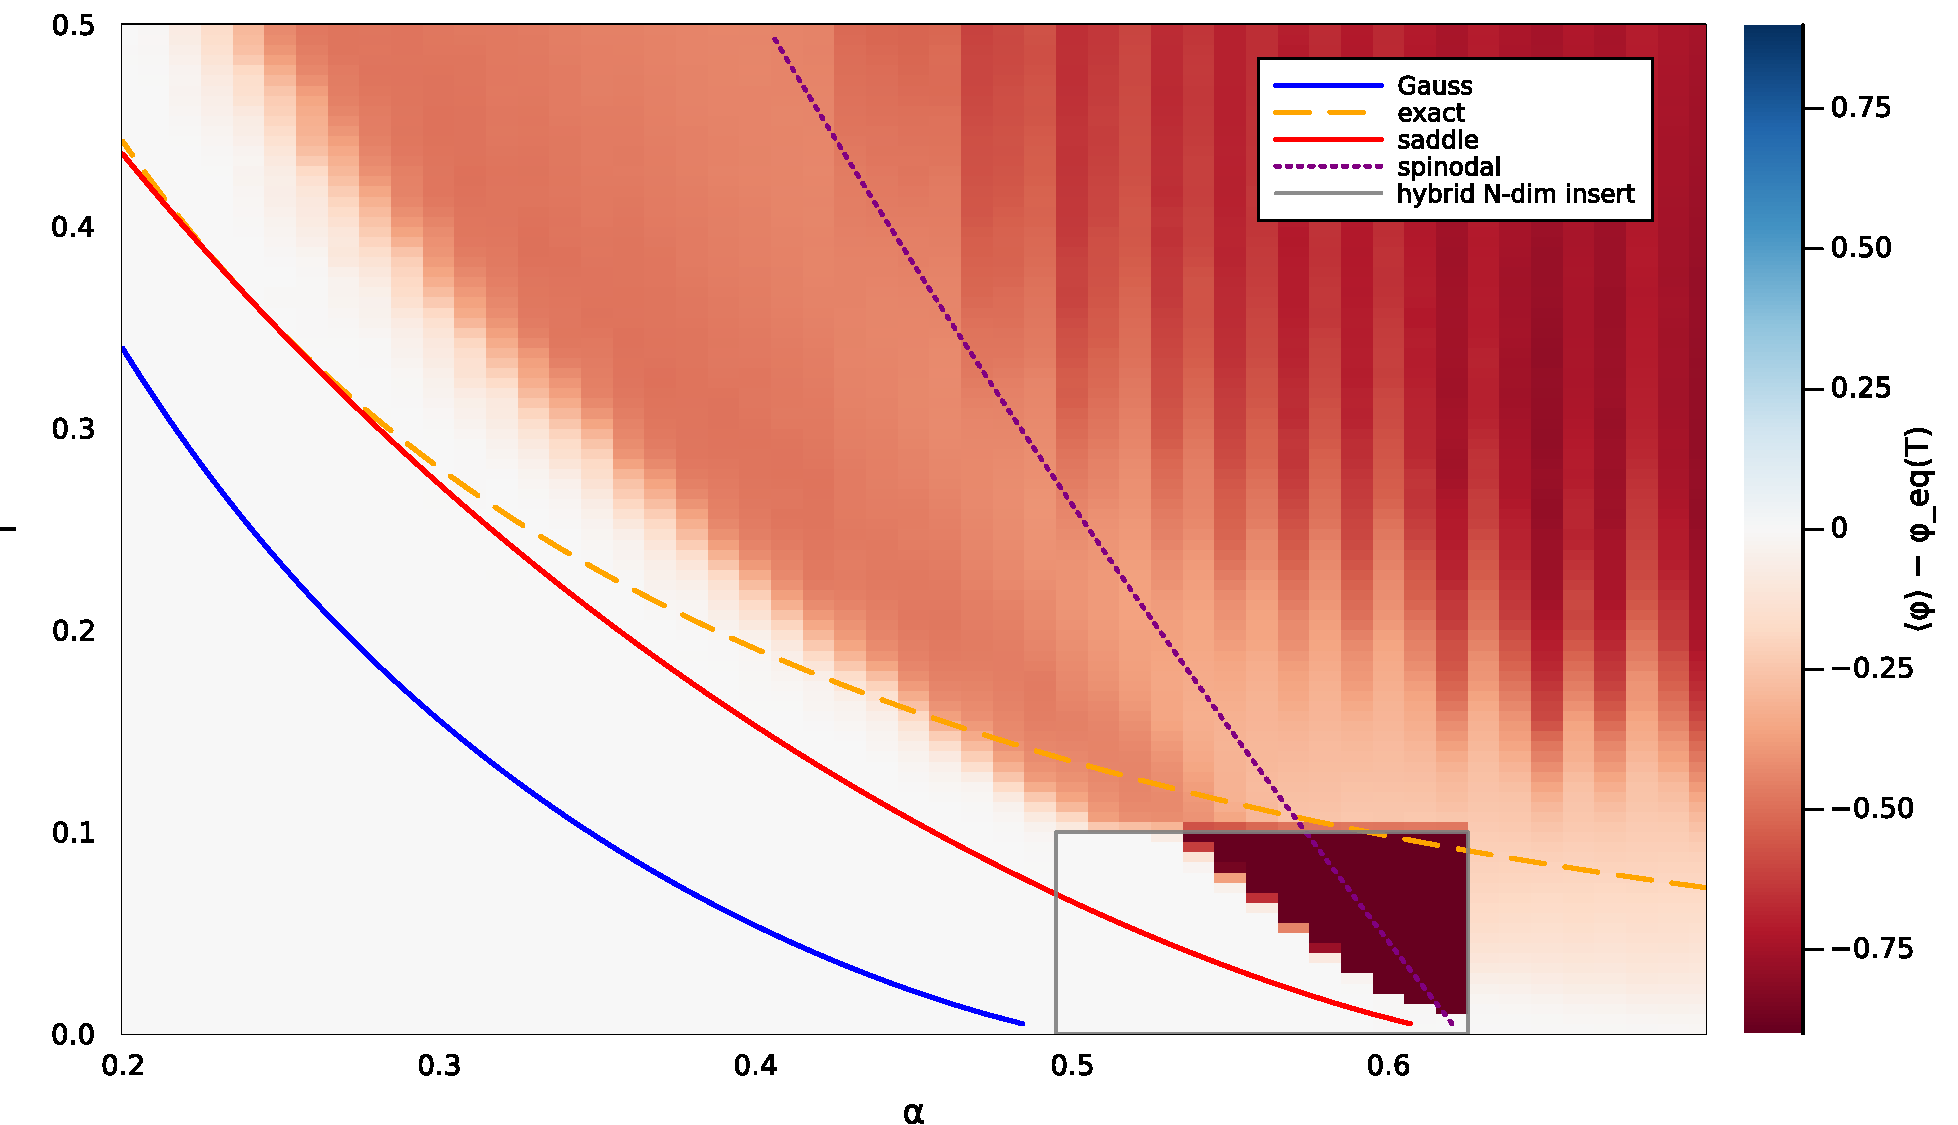
\includegraphics[width=0.95\linewidth]{panels_paper/heatmap_honest_over_Nramp_N100_Ndim.pdf}
\caption{$\avg{\varphi_1} - \phieq(T)$ from Monte Carlo over the
$(\alpha, T)$ plane at $\Bnet = 1$.  Background: truncated MC at
varying $N$ ($\alpha \in [0.20, 0.70]$, $M \approx 4.4 \times 10^6$).
Grey rectangle: N-dim hybrid MC at $N = 100$ on a fine $T$ grid.
Curves: $\acGauss$~\eqref{eq:acgauss} (blue solid, Gaussian + support
edge); $\acBd$~\eqref{eq:acbd} (orange dashed, exact density + support
edge); $\acSd$~\eqref{eq:acsd} (red solid, thermodynamic F-crossover);
$\acSp$~\eqref{eq:acsp} (purple dotted, single-pattern spinodal).
$\acSd$ and $\acSp$ share the endpoint at $T = 0$ where the basin
disappears; the empirical line at finite $N$ sits between them, on the
Kramers contour, drifting toward $\acSp$ as $N$ grows.}
\label{fig:heatmap}
\end{figure}

% =========================================================================
\section{Discussion}
\label{sec:discussion}

The Ramsauer threshold $\alpha_c = 1/2$ is a Gaussian artefact.  The
Gaussian density misses the interior saddle that the exact spherical
density places at $\varphi^{*}(\Bnet)$ in the partition-sum integrand;
restoring it gives a finite $\Bnet$-dependent capacity
$\acSd(\Bnet, 0) = \acSp(\Bnet, 0) = \Bnet - \gmax(\Bnet)$ — the load
at which the cusp $\varphi_c = (\alpha + \gmax)/\Bnet$ reaches the
unit sphere and the retrieval basin disappears.  The capacity sits
below Ramsauer's bound at moderate $\Bnet$, crosses it at
$\Bnet \approx 0.7$, and grows logarithmically beyond.  The
$\Bnet$-independence of Ramsauer's $1/2$ is itself the signature of the
right-edge replacement: at the edge the $\Bnet^{-1}$ prefactor of $H$
and the $\Bnet$ inside the exponent cancel, while at the interior
saddle the cancellation breaks through the $\Bnet$-dependence of
$\varphi^{*}$.

At $T > 0$ the saddle line $\acSd$ and the spinodal $\acSp$ separate.
$\acSd$ is the thermodynamic boundary at which the basin and the saddle
valley exchange order in free energy; $\acSp$ is the geometric boundary
at which the cusp catches the basin minimum and the retrieval branch
disappears.  For a cold-initialised chain the cusp is the only escape
route, with barrier $(\phieq - \varphi_c) + (T/2)\ln[(1 - \phieq^2)/
(1 - \varphi_c^2)]$ vanishing only at $\acSp$.  The Kramers escape time
grows exponentially in $N$ throughout $\alpha < \acSp$, irrespective of
which side of $\acSd$ the chain sits on; at $N \to \infty$ the empirical
boundary is therefore the spinodal.  At finite $N$ it is the Kramers
contour inside the strip $\acSd < \alpha < \acSp$, which is what our
hybrid MC at $N = 100$ measures.

% =========================================================================
\bibliographystyle{plainnat}
\bibliography{refs}

\end{document}
